\subsubsection{Power Calculation}
We assumed that up to rated power, the rotation of each wind turbine could be controlled such that a constant power coefficient of 0.42 was achieved. The wind turbine power generation was defined as:
\begin{equation}
P = 
\begin{cases} 
      C_P\frac{1}{2}\rho V_{\text{eff}}^3A & V_{\text{eff}}\leq V_{\text{rated}} \\
      P_{\text{rated}} & V_{\text{eff}} > V_{\text{rated}}
   \end{cases}
\end{equation}
\noindent Where $C_P$ is the power coefficient; $\rho$ is the air density which we assumed was 1.1716 kg m$^{-3}$; $A$ is the swept area of the turbine rotor; and $V_{\text{eff}}$ is an effective wind speed across rotor, which was defined as:
\begin{equation}
V_{\text{eff}} = V(1-L)
\end{equation}
\noindent Where $V$ is the free stream wind speed at the turbine hub height, and L is the total velocity deficit.


\subsubsection{Wind Speed Distributions}

We represented the speeds at any wind direction as a Weibull distribution, which is commonly used to represent wind speed distributions \citep{justus1978methods,rehman1994weibull,dorvlo2002estimating}: 
\begin{equation}
W(x) = \Big(\frac{k}{V_{\text{mean}}}\Big)\Big(\frac{x}{V_{\text{mean}}}\Big)^{k-1}\text{exp}\Big[\Big(-\frac{x}{V_{\text{mean}}}\Big)^k\Big]
\end{equation}
The shape factor, $k$, was set as 1.76. 
The mean speed for a given distribution, $V_{\text{mean}}$, could be different depending on the wind direction, meaning that each wind direction had an associated Weibull curve defining the wind speed distribution from that direction. 
Figure \ref{weibull} shows the wind speed Weibull distributions for two different $V_{\text{mean}}$ values. 


\begin{figure}[htbp]
  \centering
  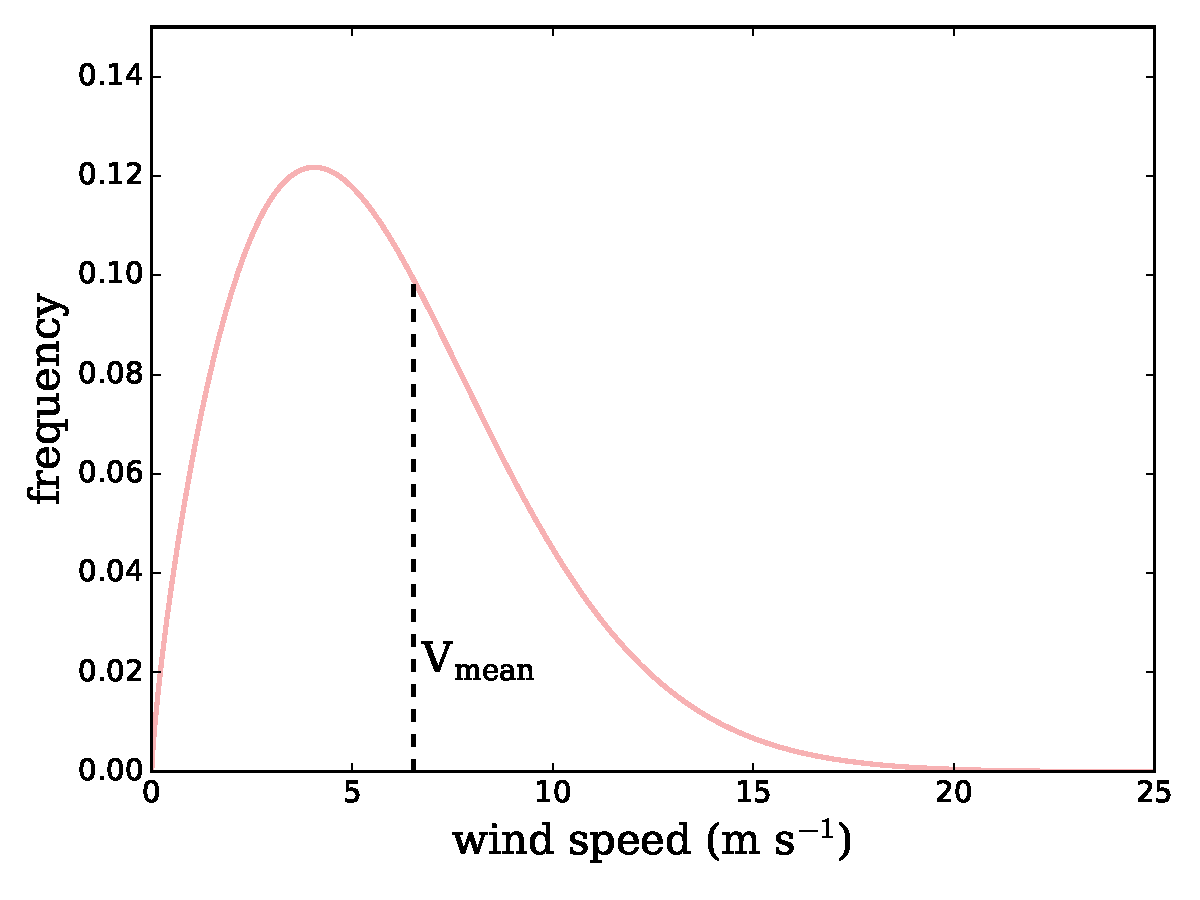
\includegraphics[trim={0 0.7cm 0 0.4cm},clip,width=0.4\textwidth]{Figures/weibull_6_53.pdf}\label{653}
  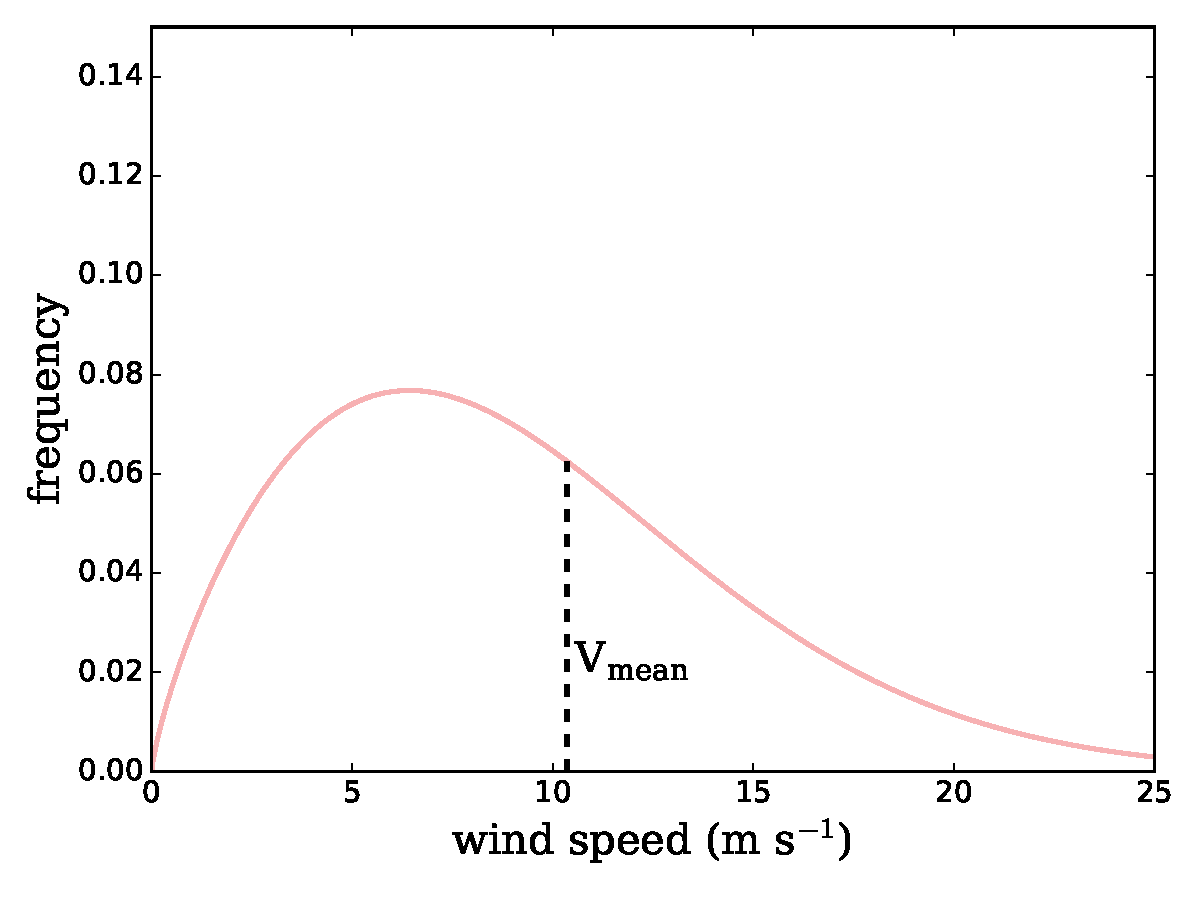
\includegraphics[trim={0 0.7cm 0 0.4cm},clip,width=0.4\textwidth]{Figures/weibull_10_35.pdf}\label{1035}
  \caption{\label{weibull} The Weibull wind speed distributions for two different average wind speeds. In (a) there is an average wind speed of 6.53 meters per second, and (b) shows an average wind speed of 10.35 meters per second. The shape factor k in each Weibull distribution was chosen as 1.76.}
\end{figure}


\subsubsection{Sampling}
The direction data we had was binned into 36 directions for one wind rose, and 72 directions for the other. This is very fine sampling;
from a convergence study, we found that it is more refined than necessary to accurately compute the annual energy production (AEP) of a wind farm. 
For every wind direction at which the power was computed, the wake model needed to be called; therefore, reducing the number of directions at which the wind farm power was computed reduced the time required to optimize. 
However, too few directions would make the AEP calculation inaccurate. We fit a spline to the direction data and were thus able to sample at any direction. We then performed a two-dimensional convergence study to find how many directions and speeds were required to approach the ``true'' AEP, which we defined to be the AEP calculated when using 50 wind directions and 30 wind speed samples. 
We found that at 23 wind direction samples and 5 wind speed samples from the Weibull distributions, the AEP converged within 2\% of the true AEP. This was within the error of our wake model; therefore, this was the number of samples used in our study. 